\mbox{$\displaystyle -\,$\,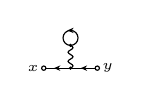
\begin{tikzpicture}[x=0.340cm, y=0.340cm, line width=0.420pt, baseline={([yshift=-0.6ex]0,0)}]
  \draw (0.000,0.000) -- (-1.000,0.000);
  \fill (-0.619,0.000) -- (-0.381,-0.102) -- (-0.458,0.000) -- (-0.381,0.102) -- cycle;
  \draw (1.000,0.000) -- (0.000,0.000);
  \fill (0.381,0.000) -- (0.619,-0.102) -- (0.542,0.000) -- (0.619,0.102) -- cycle;
  \draw plot[smooth, tension=0.7] coordinates {(0.000,0.850) (0.065,0.808) (0.092,0.765) (0.065,0.722) (0.000,0.680) (-0.065,0.638) (-0.092,0.595) (-0.065,0.552) (0.000,0.510) (0.065,0.467) (0.092,0.425) (0.065,0.382) (0.000,0.340) (-0.065,0.298) (-0.092,0.255) (-0.065,0.213) (0.000,0.170) (0.065,0.127) (0.092,0.085) (0.065,0.042) (0.000,0.000)};
  \draw (0.000,0.850) arc[start angle=270.000, end angle=630.000, radius=0.280];
  \fill (-0.119,1.410) -- (0.119,1.308) -- (0.042,1.410) -- (0.119,1.512) -- cycle;
  \fill (0.000,0.850) circle (0.064);
  \fill (0.000,0.000) circle (0.064);
  \draw[fill=white] (-1.000,0.000) circle (0.080);
  \draw[fill=white] (1.000,0.000) circle (0.080);
  \node[font=\tiny, inner sep=0pt, anchor=0] at (-1.170,0.000) {$x$};
  \node[font=\tiny, inner sep=0pt, anchor=180] at (1.170,0.000) {$y$};
\end{tikzpicture}}
\diagramgap
\mbox{$\displaystyle +\,$\,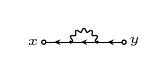
\begin{tikzpicture}[x=0.340cm, y=0.340cm, line width=0.420pt, baseline={([yshift=-0.6ex]0,0)}]
  \draw (-0.500,0.000) -- (-1.500,0.000);
  \fill (-1.119,0.000) -- (-0.881,-0.102) -- (-0.958,0.000) -- (-0.881,0.102) -- cycle;
  \draw (1.500,0.000) -- (0.500,0.000);
  \fill (0.881,0.000) -- (1.119,-0.102) -- (1.042,0.000) -- (1.119,0.102) -- cycle;
  \draw (0.500,0.000) -- (-0.500,0.000);
  \fill (-0.119,0.000) -- (0.119,-0.102) -- (0.042,0.000) -- (0.119,0.102) -- cycle;
  \draw plot[smooth, tension=0.7] coordinates {(0.500,0.000) (0.447,0.025) (0.421,0.050) (0.433,0.083) (0.468,0.130) (0.500,0.181) (0.501,0.224) (0.464,0.246) (0.404,0.247) (0.345,0.241) (0.311,0.249) (0.303,0.284) (0.311,0.342) (0.312,0.403) (0.291,0.440) (0.248,0.440) (0.196,0.410) (0.148,0.376) (0.114,0.365) (0.090,0.392) (0.067,0.446) (0.037,0.498) (0.000,0.520) (-0.037,0.498) (-0.067,0.446) (-0.090,0.392) (-0.114,0.365) (-0.148,0.376) (-0.196,0.410) (-0.248,0.440) (-0.291,0.440) (-0.312,0.403) (-0.311,0.342) (-0.303,0.284) (-0.311,0.249) (-0.345,0.241) (-0.404,0.247) (-0.464,0.246) (-0.501,0.224) (-0.500,0.181) (-0.468,0.130) (-0.433,0.083) (-0.421,0.050) (-0.447,0.025) (-0.500,0.000)};
  \fill (0.500,0.000) circle (0.064);
  \fill (-0.500,0.000) circle (0.064);
  \draw[fill=white] (-1.500,0.000) circle (0.080);
  \draw[fill=white] (1.500,0.000) circle (0.080);
  \node[font=\tiny, inner sep=0pt, anchor=0] at (-1.670,0.000) {$x$};
  \node[font=\tiny, inner sep=0pt, anchor=180] at (1.670,0.000) {$y$};
\end{tikzpicture}}
\diagramgap
\mbox{$\displaystyle -\,\frac{1}{2}$\,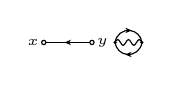
\begin{tikzpicture}[x=0.340cm, y=0.340cm, line width=0.420pt, baseline={([yshift=-0.6ex]0,0)}]
  \draw (0.900,0.000) -- (-0.900,0.000);
  \fill (-0.119,0.000) -- (0.119,-0.102) -- (0.042,0.000) -- (0.119,0.102) -- cycle;
  \draw (2.765,0.000) arc[start angle=353.974, end angle=186.026, radius=0.503];
  \fill (2.145,-0.450) -- (2.384,-0.552) -- (2.307,-0.450) -- (2.384,-0.348) -- cycle;
  \draw plot[smooth, tension=0.7] coordinates {(1.765,0.000) (1.815,0.076) (1.865,0.108) (1.915,0.076) (1.965,0.000) (2.015,-0.076) (2.065,-0.108) (2.115,-0.076) (2.165,0.000) (2.215,0.076) (2.265,0.108) (2.315,0.076) (2.365,0.000) (2.415,-0.076) (2.465,-0.108) (2.515,-0.076) (2.565,0.000) (2.615,0.076) (2.665,0.108) (2.715,0.076) (2.765,0.000)};
  \draw (1.765,0.000) arc[start angle=173.974, end angle=6.026, radius=0.503];
  \fill (2.384,0.450) -- (2.145,0.552) -- (2.223,0.450) -- (2.145,0.348) -- cycle;
  \fill (1.765,0.000) circle (0.064);
  \fill (2.765,0.000) circle (0.064);
  \draw[fill=white] (-0.900,0.000) circle (0.080);
  \draw[fill=white] (0.900,0.000) circle (0.080);
  \node[font=\tiny, inner sep=0pt, anchor=0] at (-1.070,0.000) {$x$};
  \node[font=\tiny, inner sep=0pt, anchor=180] at (1.070,0.000) {$y$};
\end{tikzpicture}}
\diagramgap
\mbox{$\displaystyle +\,\frac{1}{2}$\,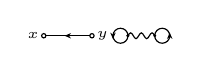
\begin{tikzpicture}[x=0.340cm, y=0.340cm, line width=0.420pt, baseline={([yshift=-0.6ex]0,0)}]
  \draw (0.900,0.000) -- (-0.900,0.000);
  \fill (-0.119,0.000) -- (0.119,-0.102) -- (0.042,0.000) -- (0.119,0.102) -- cycle;
  \draw plot[smooth, tension=0.7] coordinates {(2.245,0.000) (2.295,0.076) (2.345,0.108) (2.395,0.076) (2.445,0.000) (2.495,-0.076) (2.545,-0.108) (2.595,-0.076) (2.645,0.000) (2.695,0.076) (2.745,0.108) (2.795,0.076) (2.845,0.000) (2.895,-0.076) (2.945,-0.108) (2.995,-0.076) (3.045,0.000) (3.095,0.076) (3.145,0.108) (3.195,0.076) (3.245,0.000)};
  \draw (2.245,0.000) arc[start angle=0.000, end angle=360.000, radius=0.280];
  \fill (1.685,-0.119) -- (1.787,0.119) -- (1.685,0.042) -- (1.583,0.119) -- cycle;
  \draw (3.245,0.000) arc[start angle=180.000, end angle=540.000, radius=0.280];
  \fill (3.805,0.119) -- (3.703,-0.119) -- (3.805,-0.042) -- (3.907,-0.119) -- cycle;
  \fill (2.245,0.000) circle (0.064);
  \fill (3.245,0.000) circle (0.064);
  \draw[fill=white] (-0.900,0.000) circle (0.080);
  \draw[fill=white] (0.900,0.000) circle (0.080);
  \node[font=\tiny, inner sep=0pt, anchor=0] at (-1.070,0.000) {$x$};
  \node[font=\tiny, inner sep=0pt, anchor=180] at (1.070,0.000) {$y$};
\end{tikzpicture}}
